%%%%
\subsection{Scheduler plugin input}\label{s:ExperimentSetup:Input}

% \todo{Opisać input algorytmów schedulingu, jak zostały wyznaczone wartości, zaprezentować same plany wykonania po wykonaniach algorytmów}

% \todo{dopisz tytulem wstepu ze korzystamy z pluginu - hetf i peft}

The scheduling solution presented in this work creates a plan of workflow execution with either HEFT or PEFT scheduling algorithms. 
Data required for input by both algorithms used in the scheduler has the same format.
It comprises of two matrices, one filled with computation costs and another with communication costs.
The costs of computation have to be provided separately for each task and each processing unit in the cluster.
As for communication costs, they need to be provided for each pair of processors.

In the conducted experiments, a few assumptions were made during the input matrix composition.
The execution time for each task, excluding the time overhead spent on containerization, was taken as a task computation cost.
As the cluster is composed of nodes with only two possible different instance types, it also has been assumed that the task execution times should be the same for each processor within a single node group.
Thus, only two execution times were provided for every task, one for each node group in the cluster:

% \medskip
% \begin{minipage}{0.65\textwidth}
% {\footnotesize Depicts Kubernetescluster components and processes distributed among them.\par}
% \end{minipage}
\begin{align}
C_{comp}=
\begin{bmatrix}
T_{0, 0} & T_{0, 1} & \dots & T_{0, j}\\
T_{1, 0} & \ddots &  & \\
\vdots &  & \ddots & \\
T_{i, 0} &  &  & T_{i, j}\\
\end{bmatrix}.
\end{align}

\begin{center}
\medskip
\begin{minipage}{0.5\textwidth}
% \centering
\small
$C_{comp}$ -- computation cost matrix

$T_{i, j}$ -- time to execute \emph{i-th} task on \emph{j-th} processor
\end{minipage}
\medskip
\end{center}
% \begin{bmatrix}
% 1 & 2 & 3\\
% a & b & c
% \end{bmatrix}
As all cluster nodes are located within a single network managed within a single data centre, it was assumed that the communication cost should be the same for each processor pair.
The only exception was the communication of a processing unit with itself, which was assumed to have no cost:


\begin{align}
C_{comm}=
\begin{bmatrix}
0 & 1 & \dots & 1\\
1 & \ddots &  & \vdots \\
\vdots &  & \ddots & 1 \\
1 & \dots & 1 & 0 \\
\end{bmatrix}.
\end{align}

\begin{center}
\medskip
\begin{minipage}{0.6\textwidth}
\small
$C_{comm}$ -- communication cost matrix form experiment setup
\end{minipage}
\medskip
\end{center}

% In conducted experiments we set all the values

% \todo{Dodaj obrazki planow wykonania workflow 3x HEFTT i PEFT}

%%%%%
\begin{figure}[H]
\begin{subfigure}{1.0\textwidth}
\centering
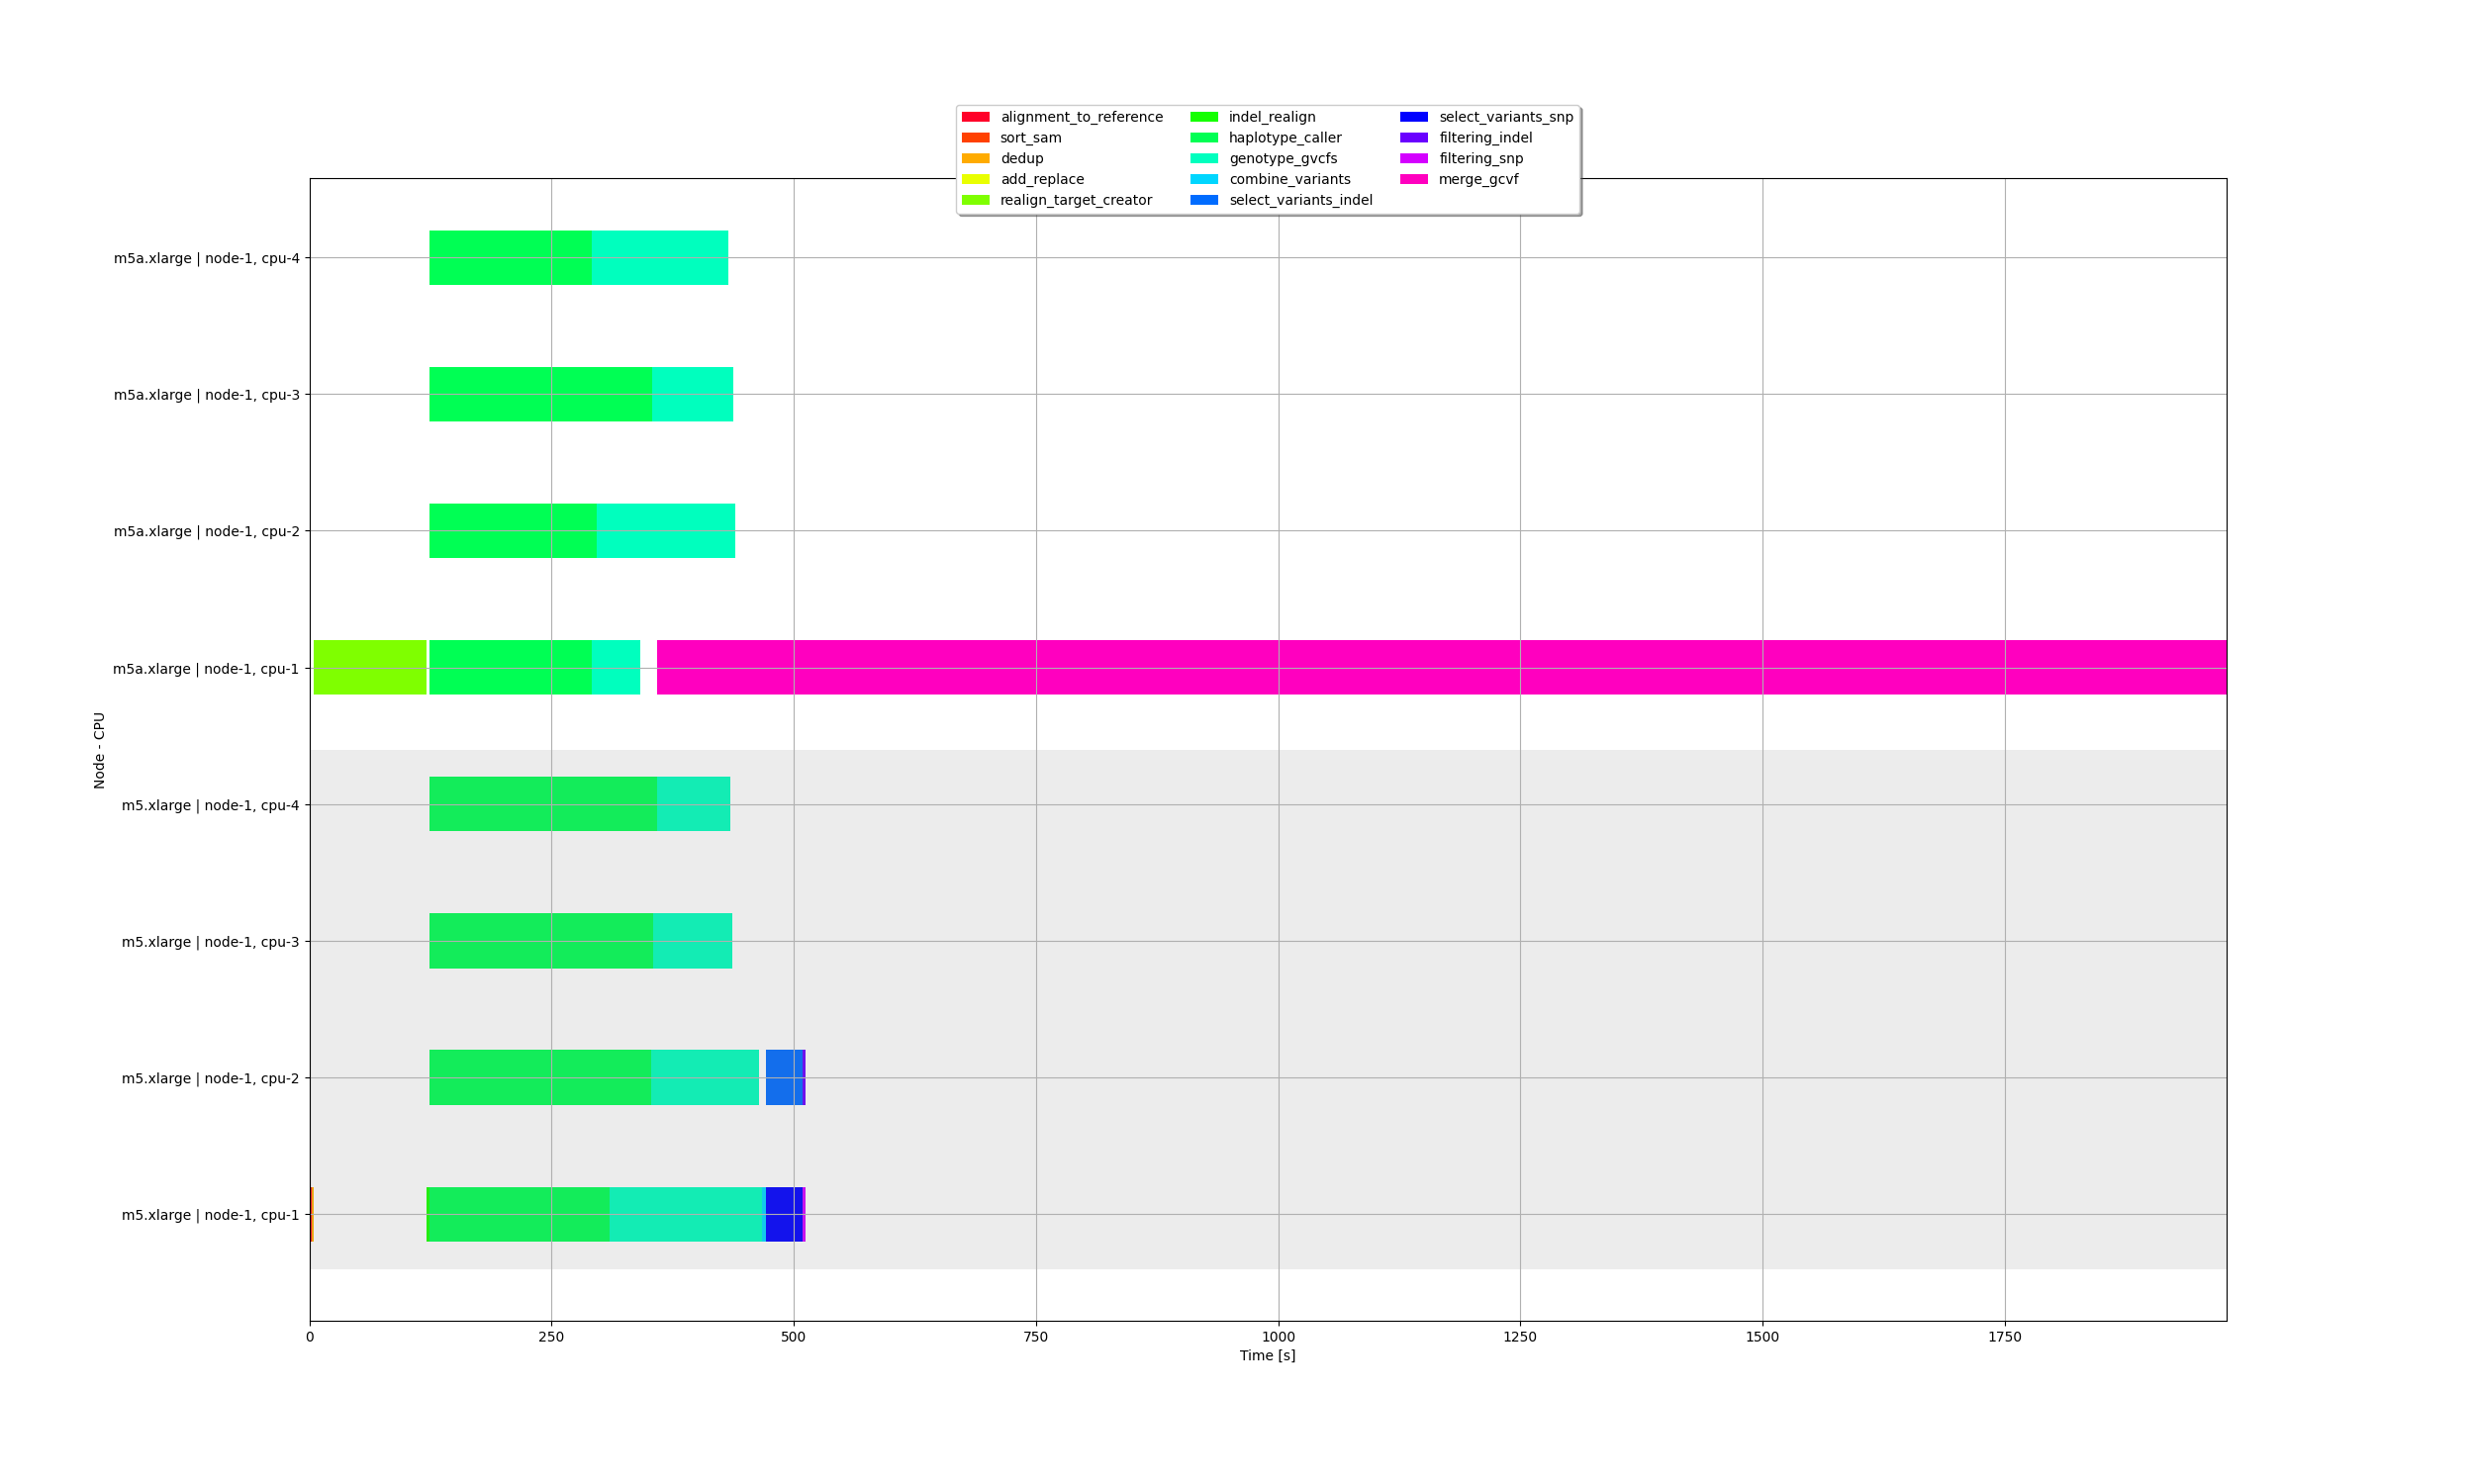
\includegraphics[width=1\linewidth]{figures/5-2-soykb_heft.png}
\caption[Schedules computed for SoyKB workflow - HEFT]{HEFT}
\label{fig:setup-input:soykb:heft}
\end{subfigure}
\begin{subfigure}{1.0\textwidth}
\centering
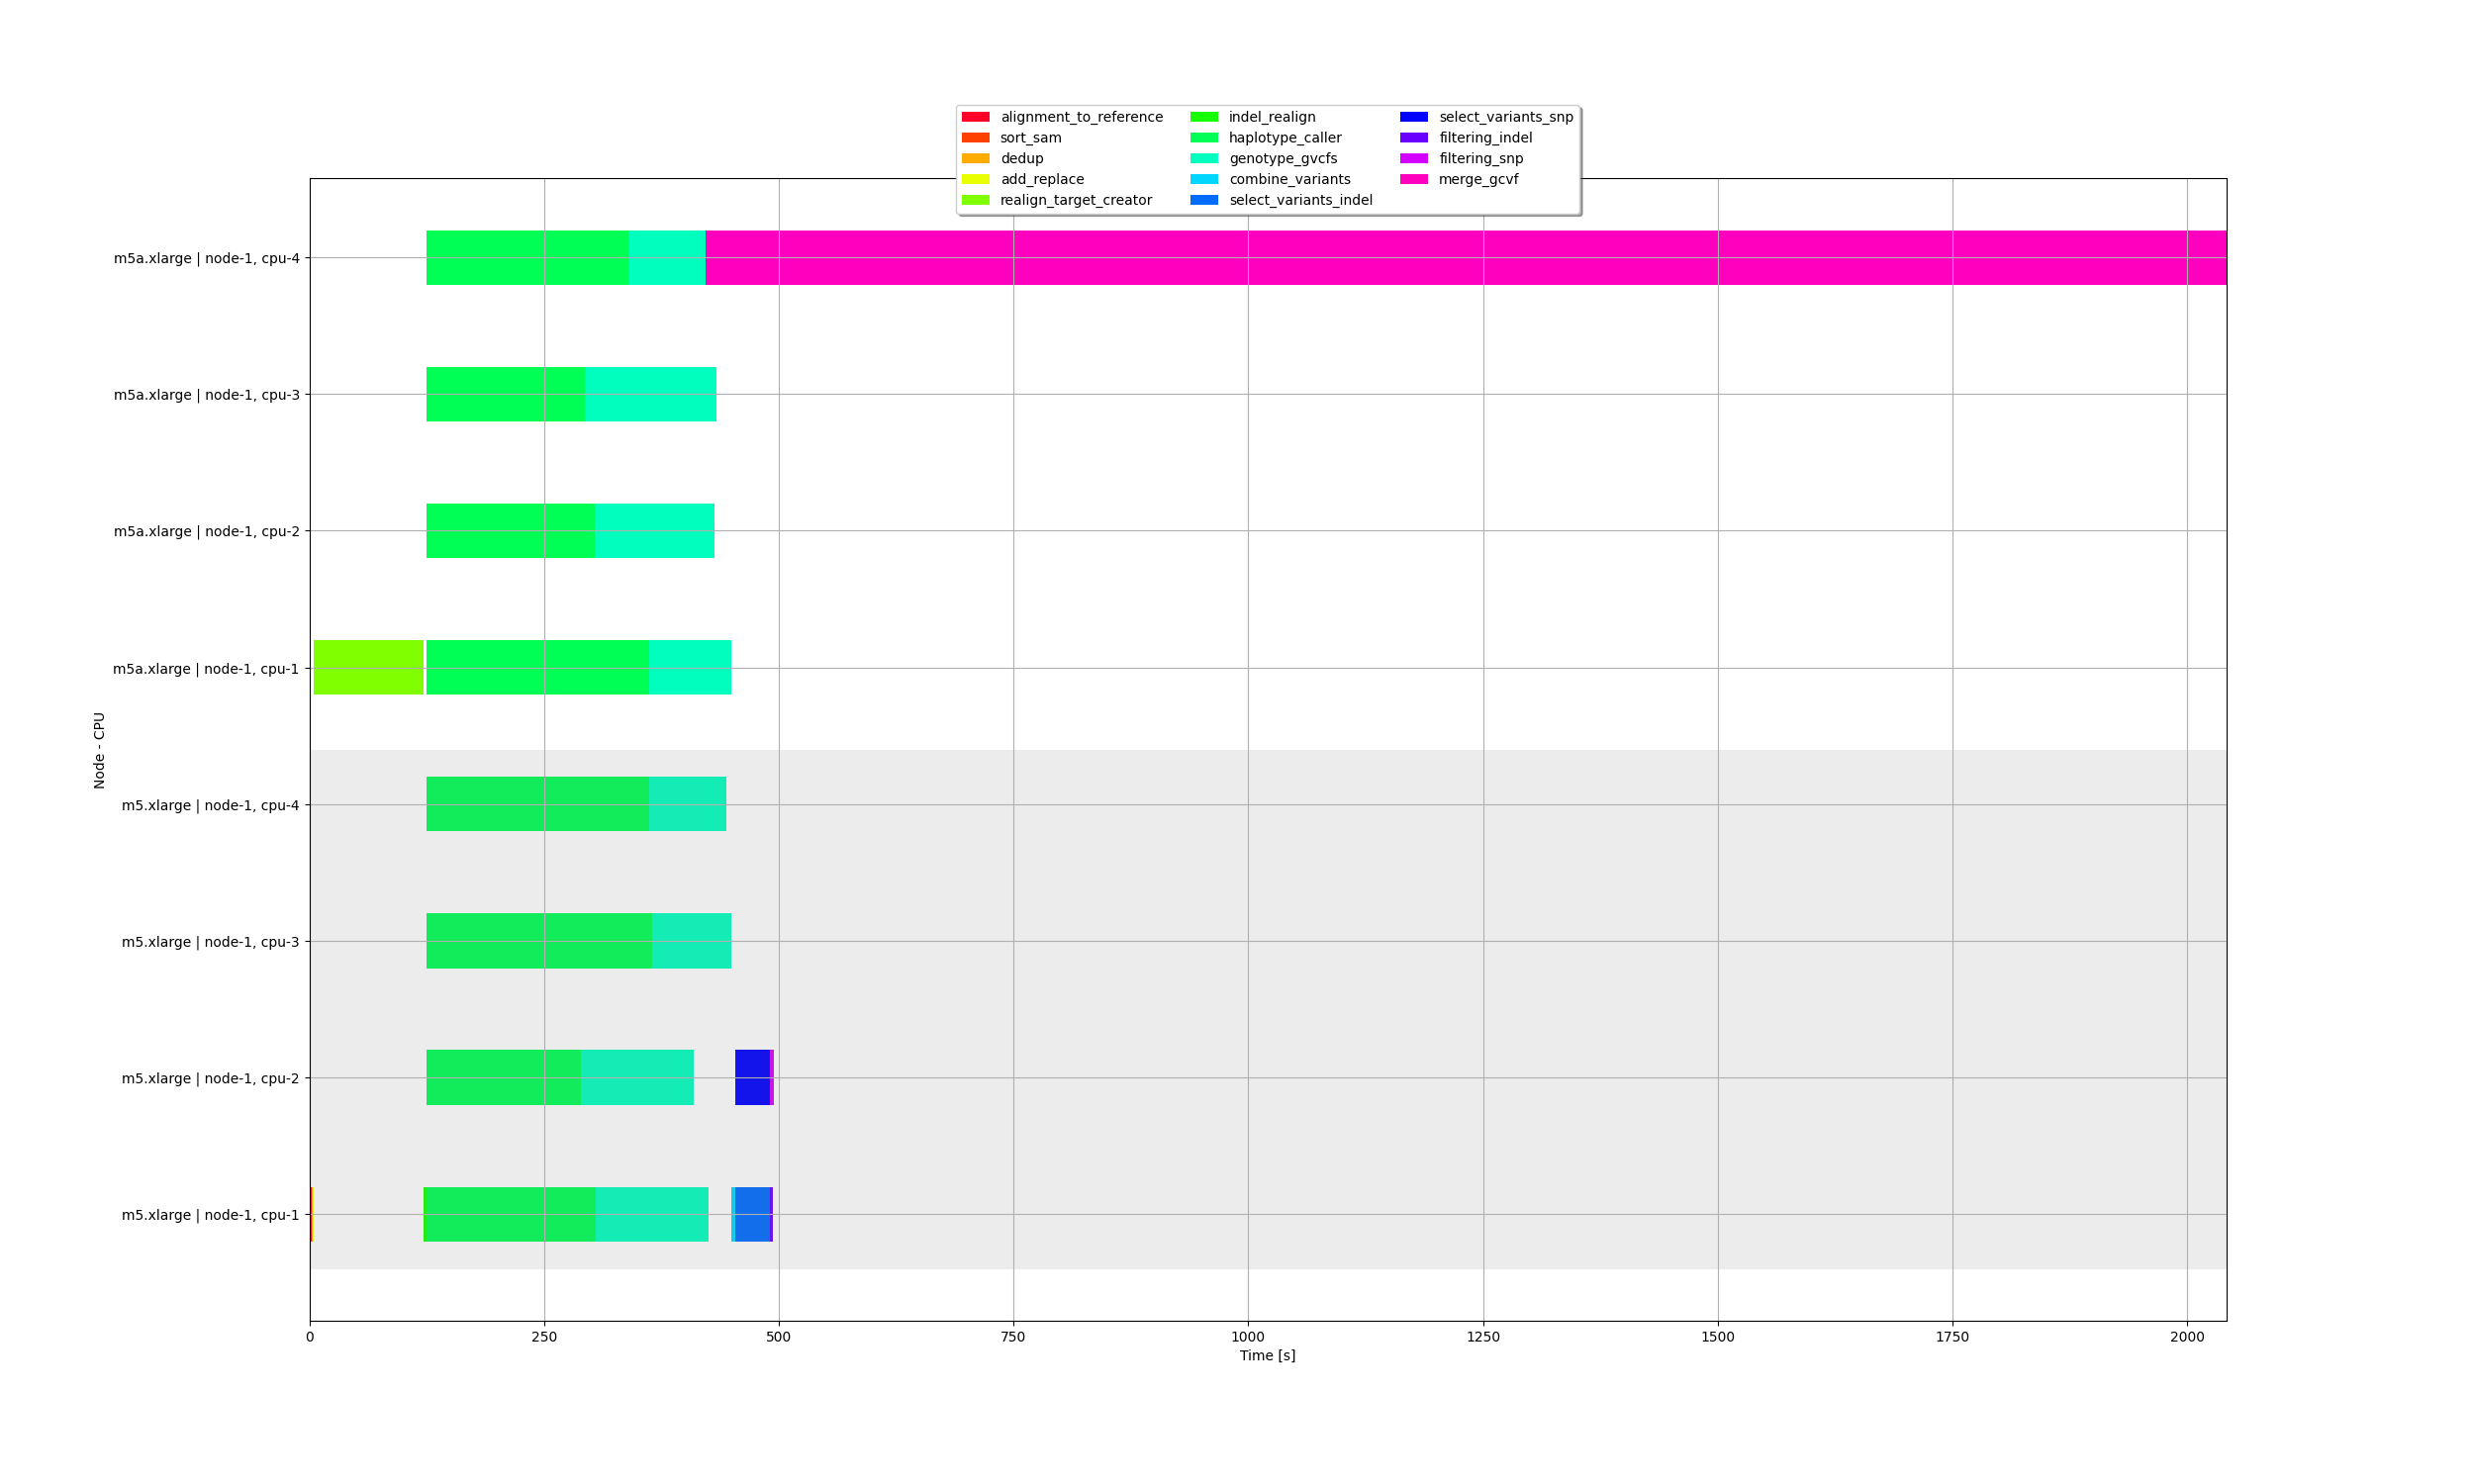
\includegraphics[width=1\linewidth]{figures/5-2-soykb_peft.png}
\caption[Schedules computed for SoyKB workflow - PEFT]{PEFT}
\label{fig:setup-input:soykb:peft}
\end{subfigure}
\centering
%%
\caption[Schedules computed for SoyKB workflow]{Schedules computed for SoyKB workflow}
\label{fig:setup-input:soykb}
\end{figure}
%%%%%

%%%%%
\begin{figure}[H]
\begin{subfigure}{1.0\textwidth}
\centering
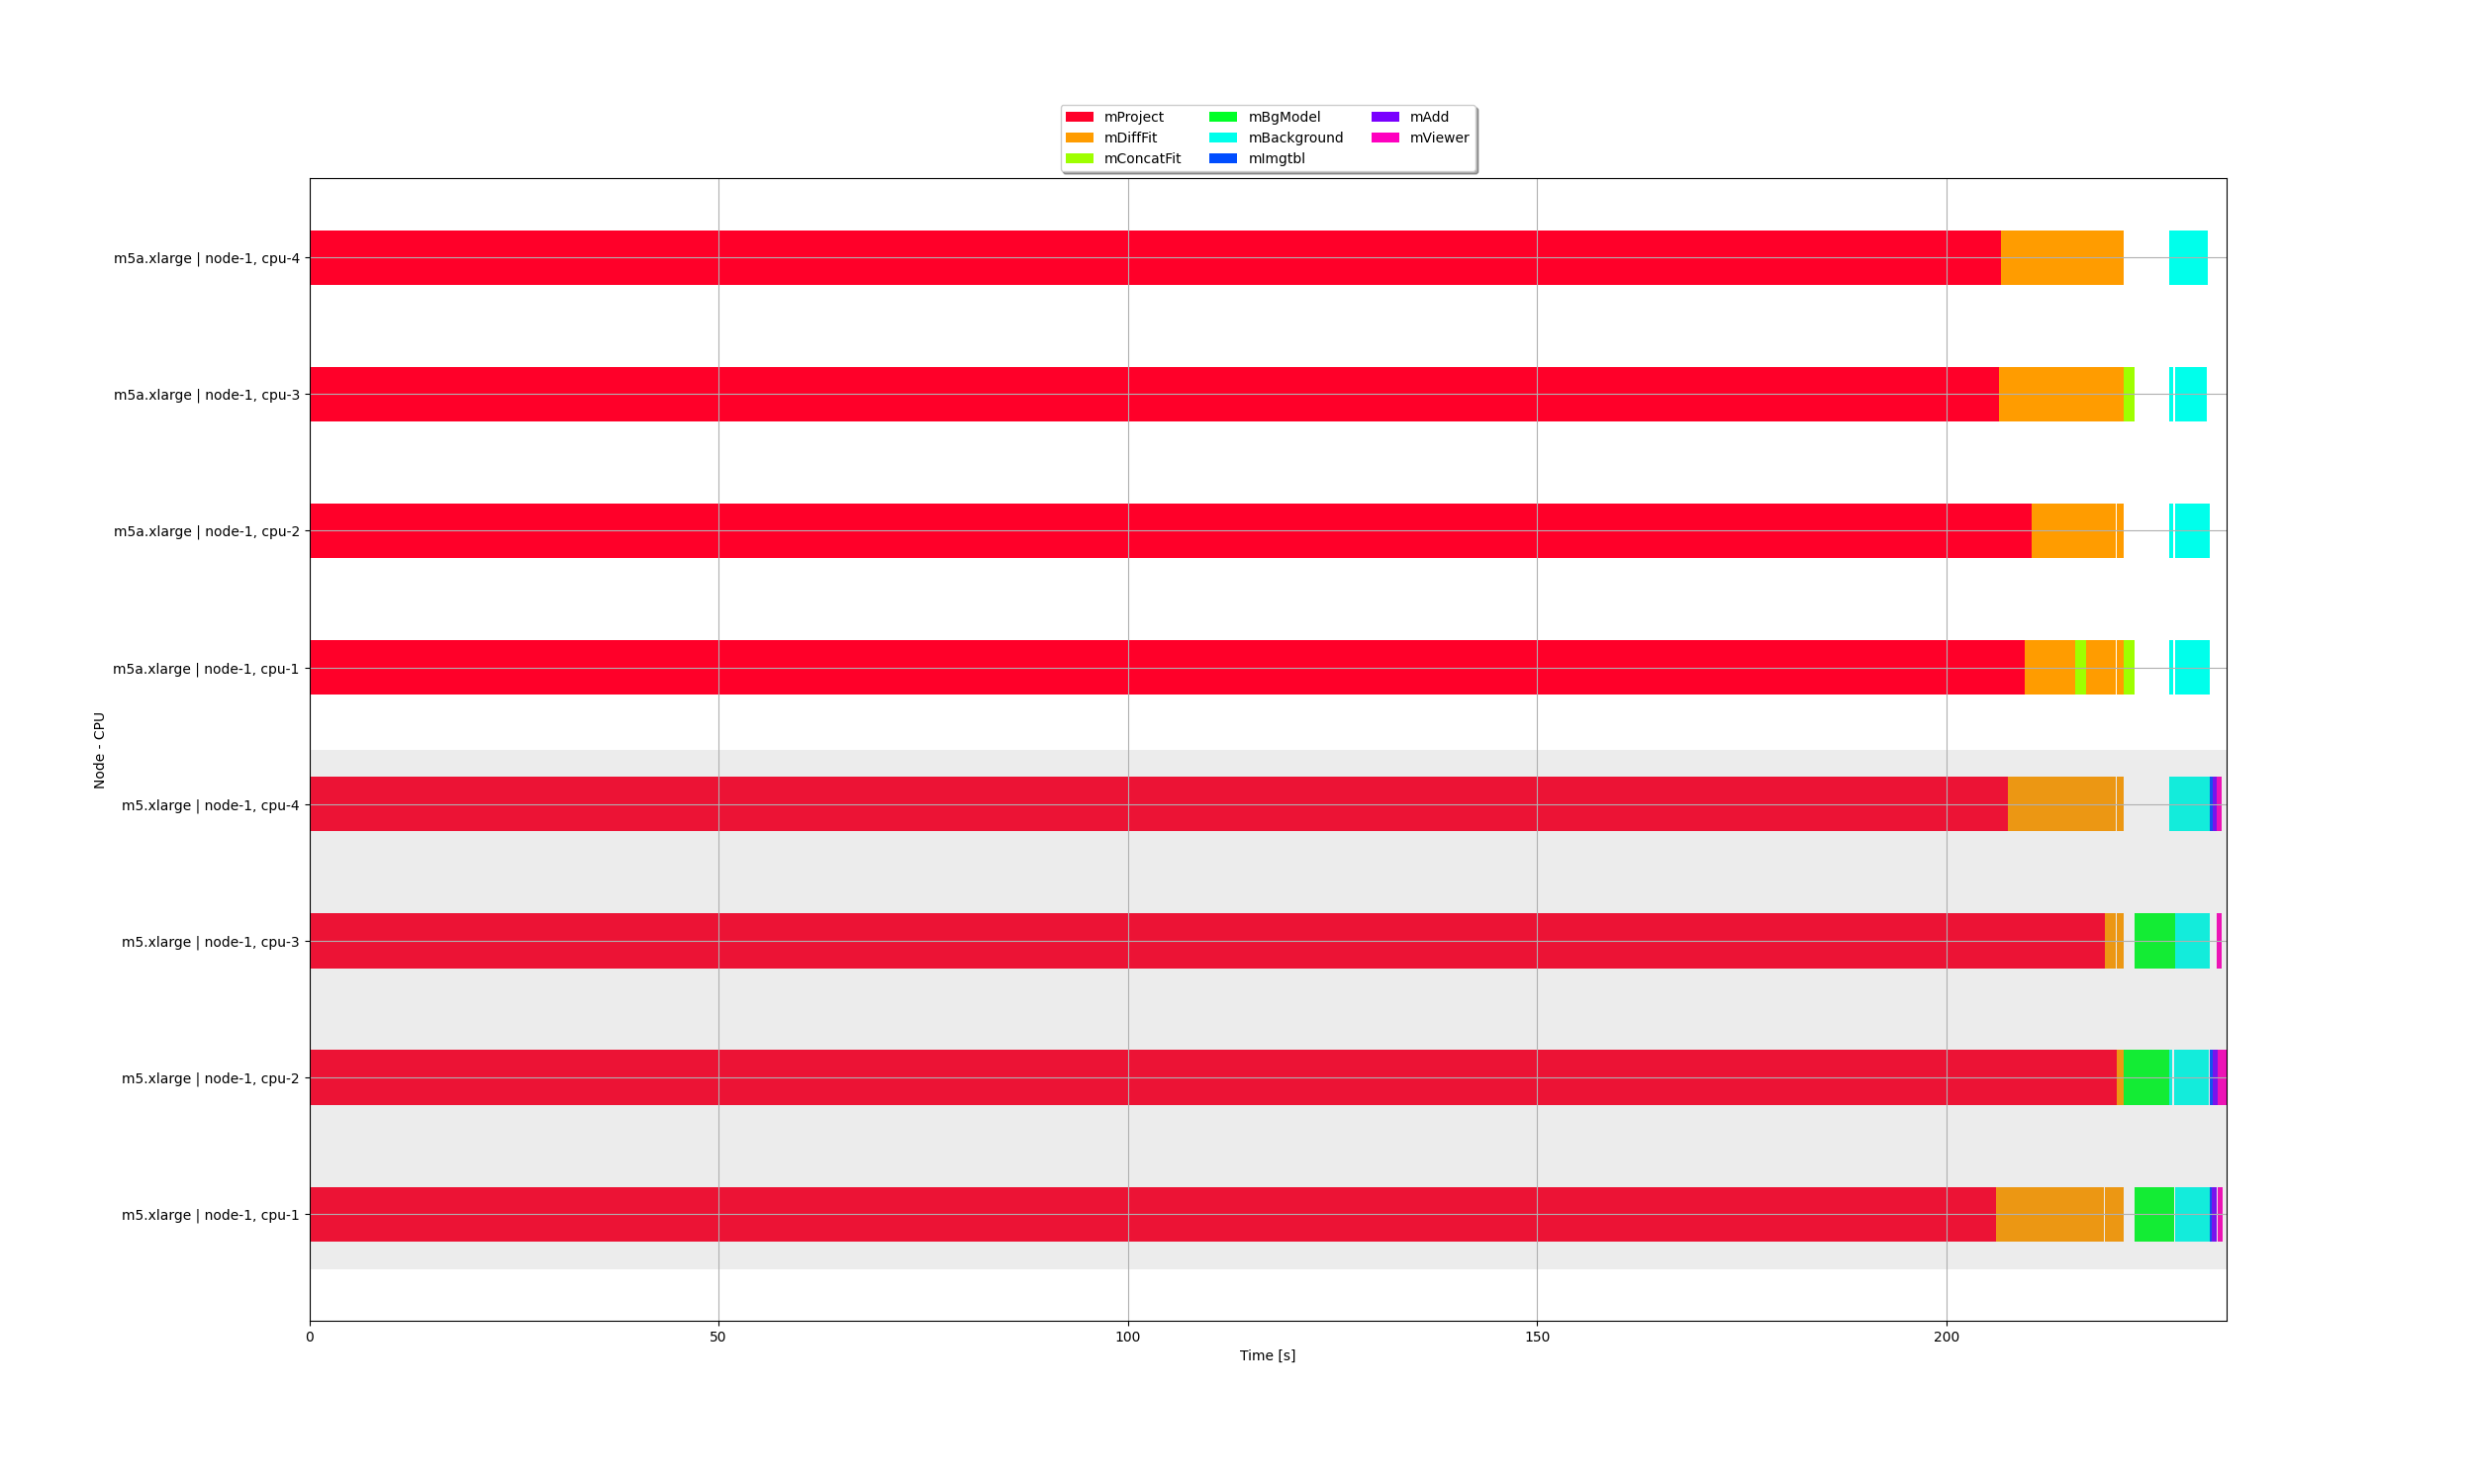
\includegraphics[width=1\linewidth]{figures/5-2-montage025_heft.png}
\caption[Schedules computed for Montage2-v0.25 workflow - HEFT]{HEFT}
\label{fig:setup-input:m025:heft}
\end{subfigure}
\begin{subfigure}{1.0\textwidth}
\centering
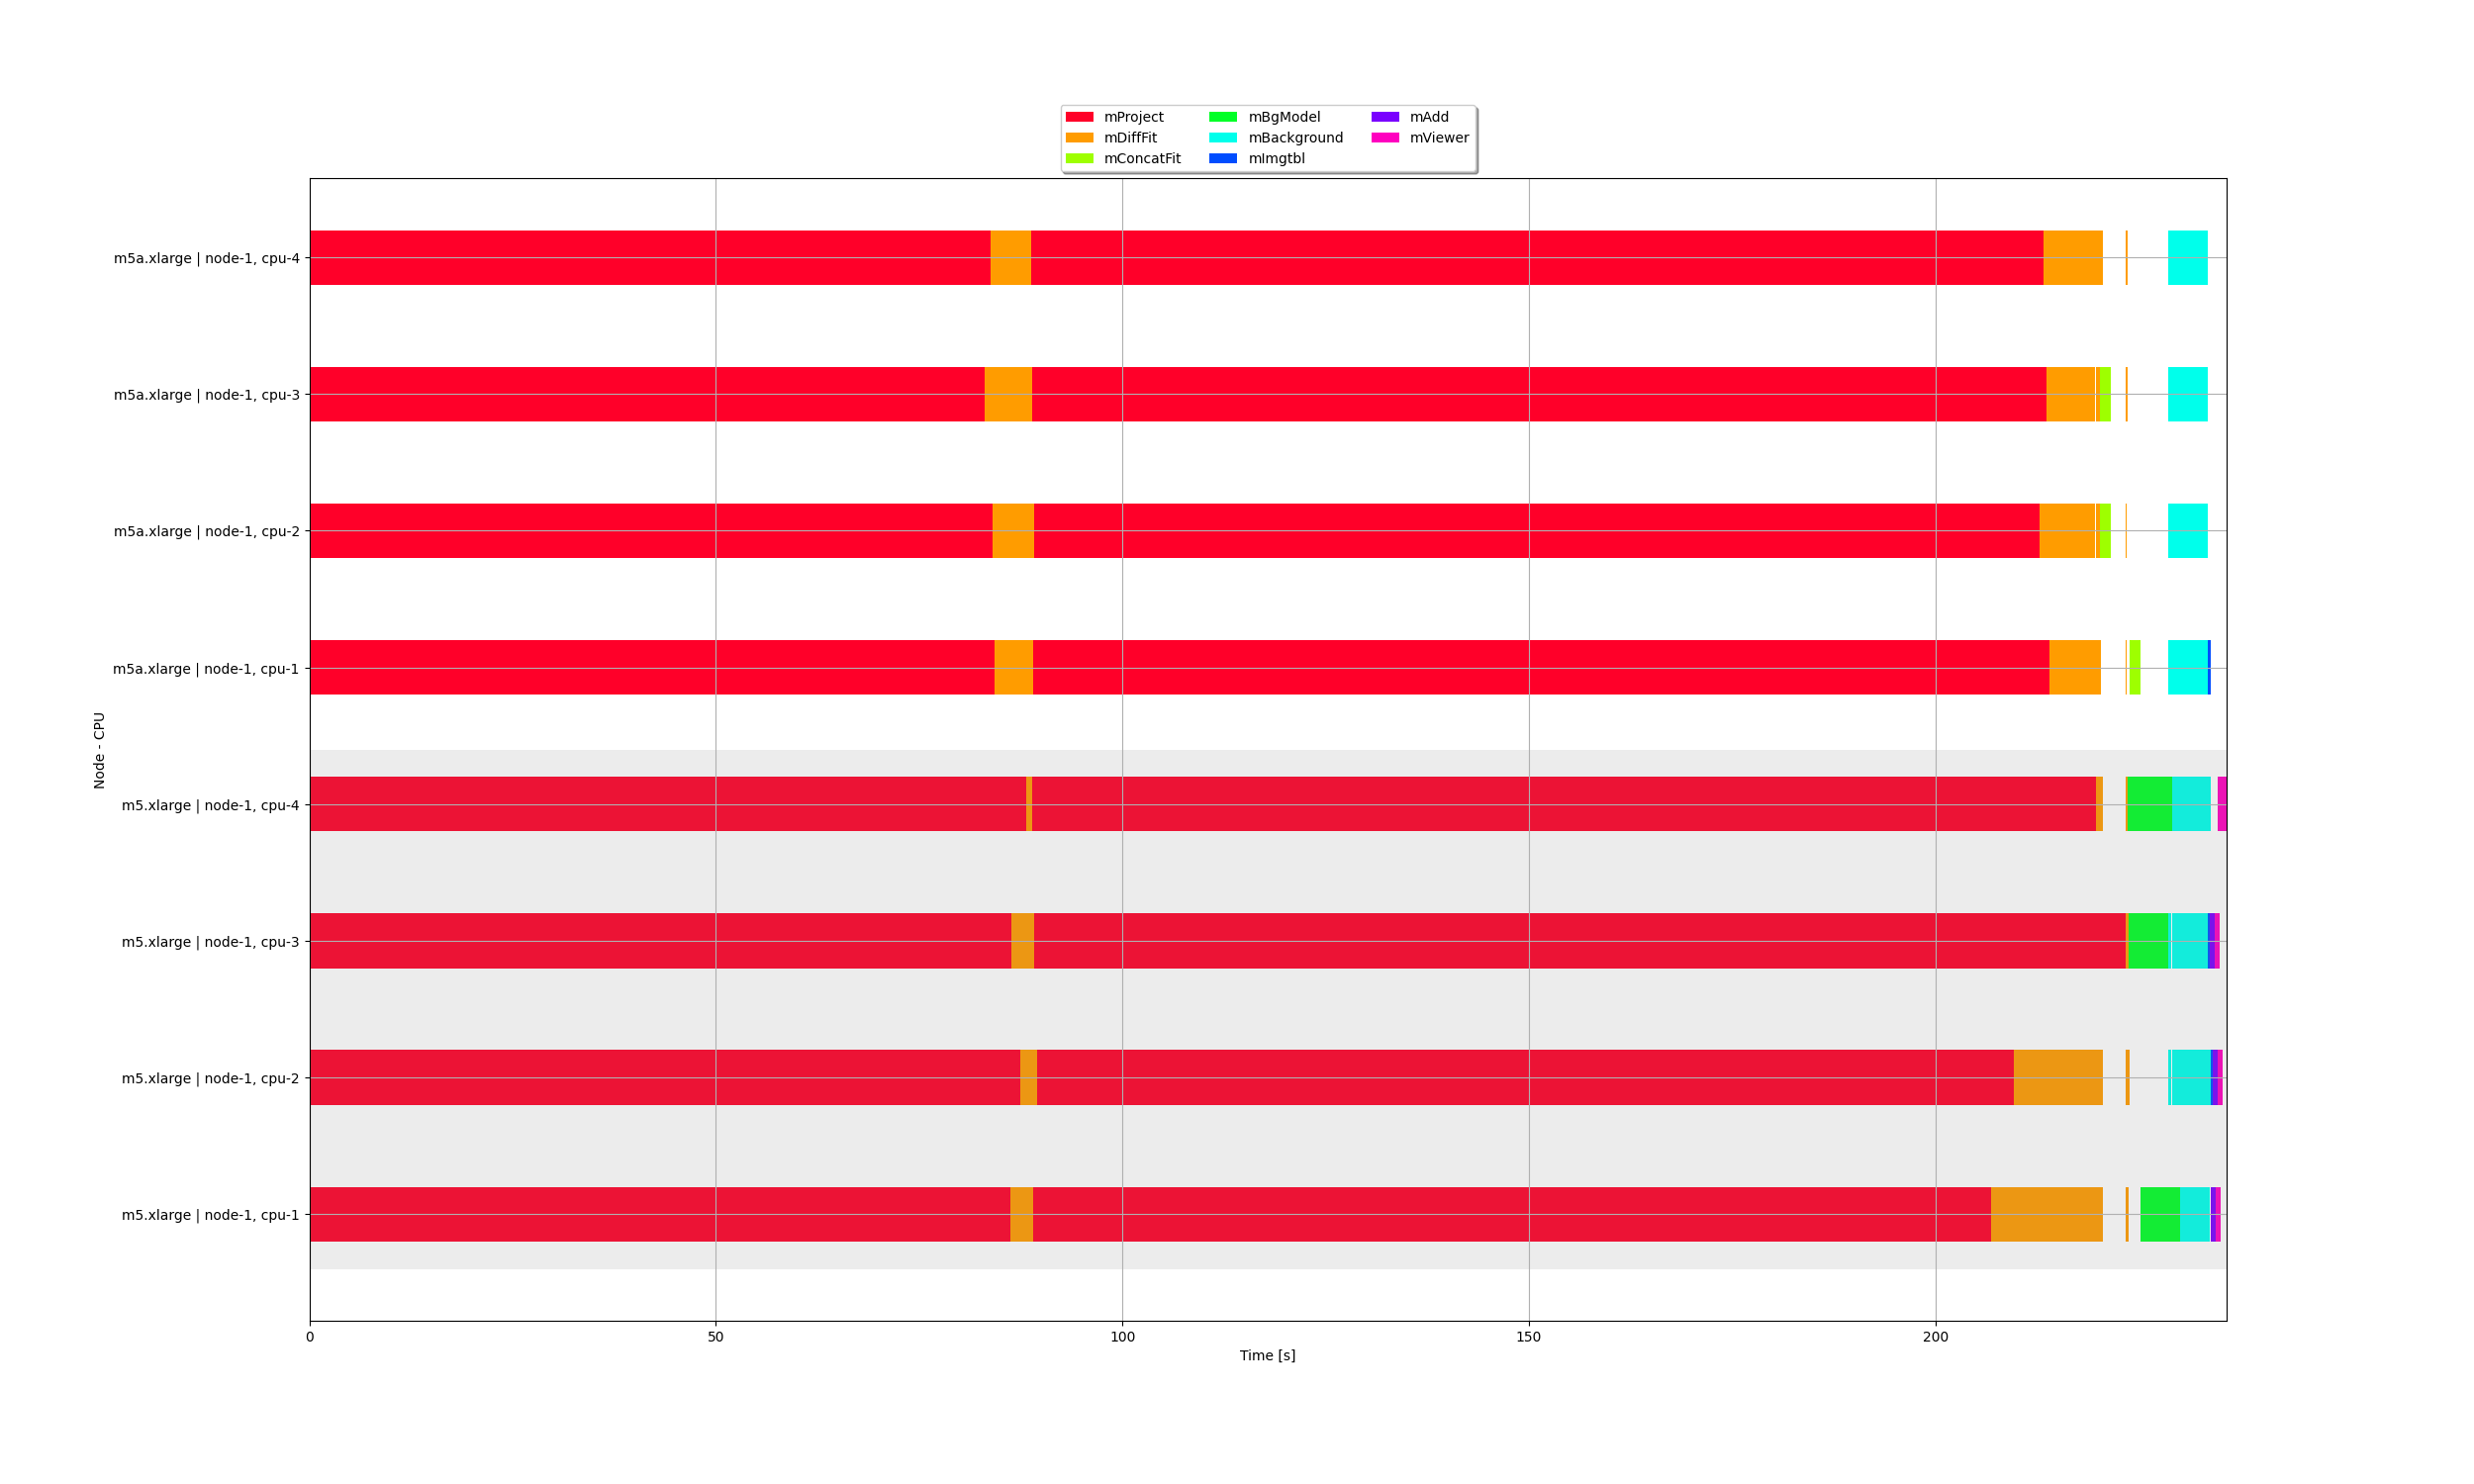
\includegraphics[width=1\linewidth]{figures/5-2-montage025_peft.png}
\caption[Schedules computed for Montage2-v0.25 workflow - PEFT]{PEFT}
\label{fig:setup-input:m025:peft}
\end{subfigure}
\centering
%%
\caption[Schedules computed for Montage2-v0.25 workflow]{Schedules computed for Montage2-v0.25 workflow}
\label{fig:setup-input:m025}
\end{figure}
%%%%%

%%%%%
\begin{figure}[H]
\begin{subfigure}{1.0\textwidth}
\centering
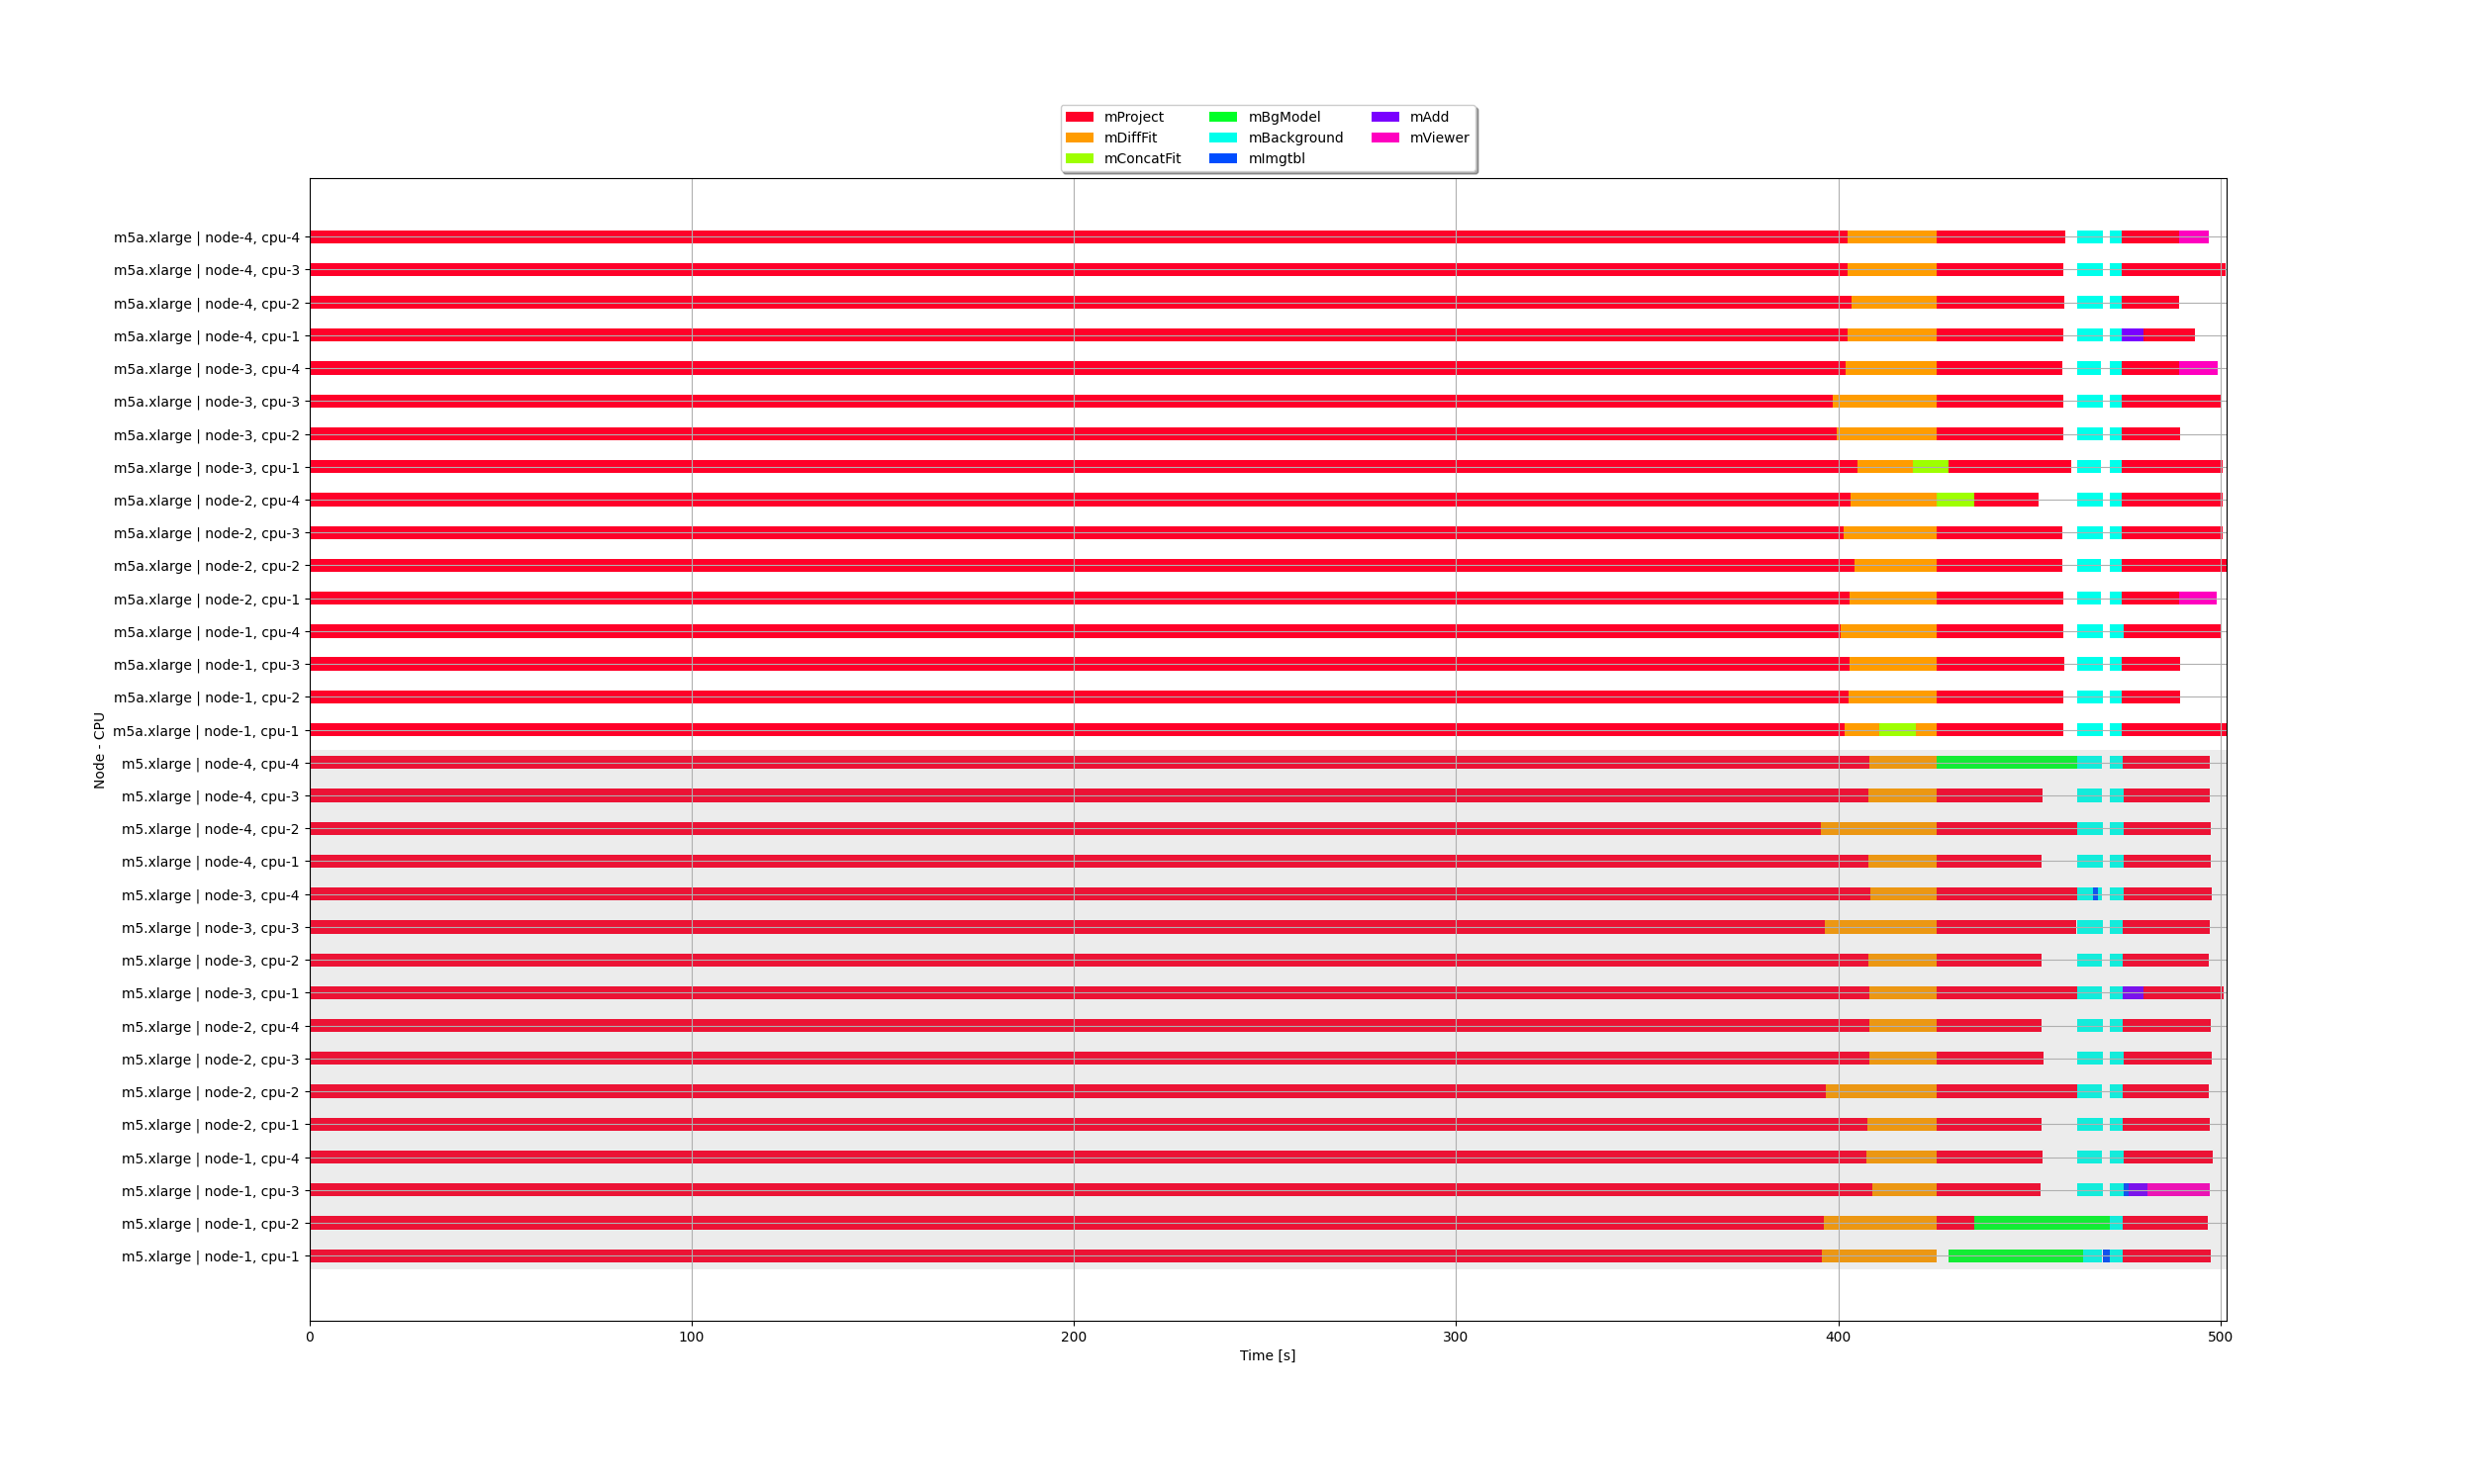
\includegraphics[width=1\linewidth]{figures/5-2-montage10_heft.png}
\caption[Schedules computed for Montage2-v1.0 workflow - HEFT]{HEFT}
\label{fig:setup-input:m10:heft}
\end{subfigure}
\begin{subfigure}{1.0\textwidth}
\centering
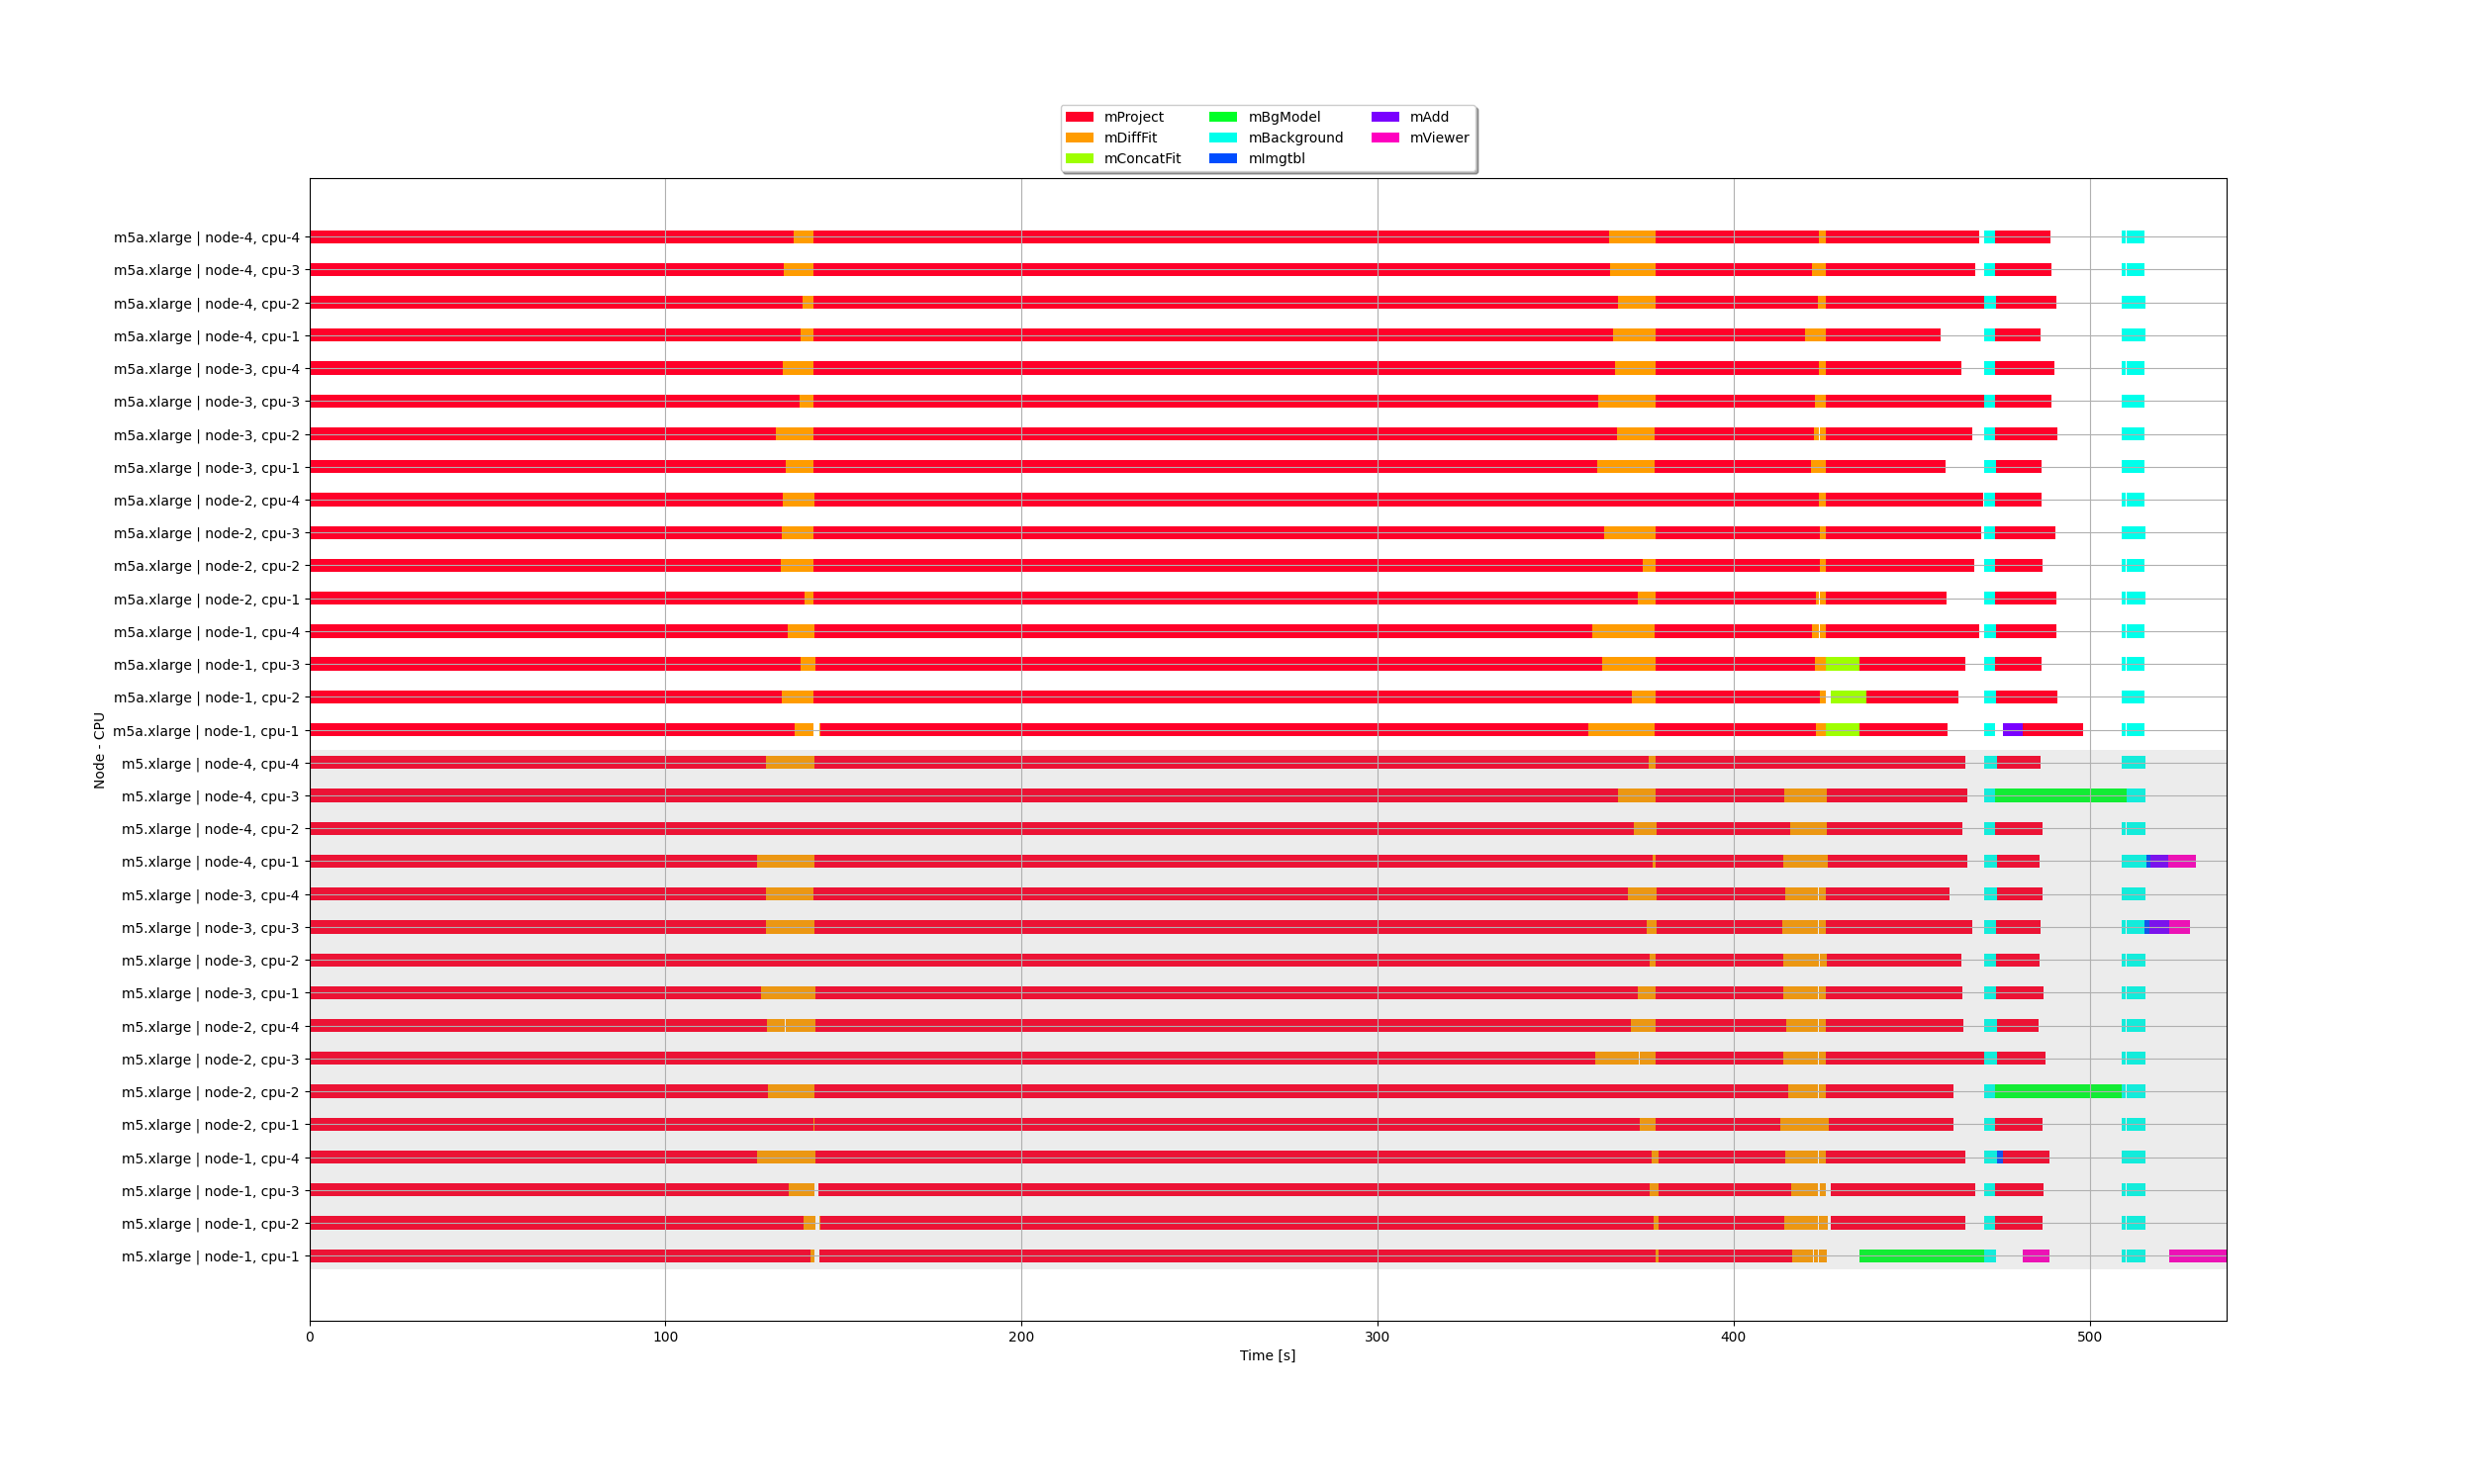
\includegraphics[width=1\linewidth]{figures/5-2-montage10_peft.png}
\caption[Schedules computed for Montage2-v1.0 workflow - PEFT]{PEFT}
\label{fig:setup-input:m10:peft}
\end{subfigure}
\centering
%%
\caption[Schedules computed for Montage2-v1.0 workflow]{Schedules computed for Montage2-v1.0 workflow}
\label{fig:setup-input:m10}
\end{figure}
%%%%%


